\chapter{Beschreibung der verschiedenen Messungen und Ergebnisdarstellung}

\section{Part 1}


\subsection{Konfiguration der Hosts}\label{hostconfig}

Zun�chst werden die Host mit statischen IP-Adressen konfiguriert:

\begin{itemize}
  \item Host 1
  	\begin{itemize}
    	\item IP-Adresse: 172.16.0.2
    	\item Subnetz-Maske: 255.255.0.0
    	\item Default Gateway: 172.16.0.1
    \end{itemize}
  \item Host 2
  	\begin{itemize}
    	\item IP-Adresse: 172.18.0.2
    	\item Subnetz-Maske: 255.255.0.0
    	\item Default Gateway: 172.18.0.1
    \end{itemize}
\end{itemize}

\subsection{Konfiguration der Router}

\subsubsection{Basis-Einstellungen}

Bei beiden Routern ist zun�chst der \textbf{Hostname} zu �ndern. Dies geschieht
�ber den Global Configuration Mode. Mit dem Kommando \textit{hostname R1} bzw.
\textit{hostname R2} werden die Hostnamen zu R1 bzw. R2 ge�ndert.
\newline
Danach werden die \textbf{Passw�rter} (console und vty) konfiguriert und
aktiviert.%TODO Ausz�ge
\newline
Es folgt die Konfiguration eines \textbf{\acs{MOTD}}-Banners:
%TODO Auszug
\newline
Um zu gew�hrleisten, dass die Router \textbf{keine Namensaufl�sung via
DNS-Server} betreiben, wird das Kommando \textit{no ip domain lookup} genutzt.
\newline
%TODO logging synchronous

\paragraph{Running Configuration}\mbox{} \\
Die Ausgabe der running-config zeigt folgendes bzgl. der konfigurierten
Passw�rter:

\begin{lstlisting}
enable secret 5 $1$r.BO$ZHkNZfQvcrvrVhJWWQDtg/
enable password cisco
\end{lstlisting}

Das Passwort f�r den allgemeinen Routerzugriff ist entschl�sselt in der
Konfigurations-Datei zu finden. Verschl�sselt hingegen ist das Passwort f�r den
Priviliedged EXEC Mode. Weitere Passw�rter sind in dieser Datei nicht zu finden.

\clearpage

\subsubsection{Konfiguration der Serial Interfaces}

Den Routern R1 und R2 m�ssen die jeweiligen IP-Adressen des Serial Interfaces
zugewiesen werden:

\begin{lstlisting}
R1(config)#interface serial 0/0/0
R1(config-if)#description WAN link to R2
R1(config-if)#ip address 172.17.0.1 255.255.0.0
R1(config-if)#clock rate 64000
R1(config-if)#no shutdown
R1(config-if)#exit
R1(config)#exit
\end{lstlisting}

R1 wird 172.17.0.1 zugewiesen. Die Clock Rate muss nur an dem Router
konfiguriert werden, mit dem die DCE-Schnittstelle des Serial-Kabels verbunden
ist (in diesem Fall R1).
\newline
\newline
\underline{Informationen des Serial Interfaces von R1:}
\newline
\newline
Durch das Kommando \textit{show interfaces serial 0/0/0} erh�lt man folgende
Informationen �ber die durchgef�hrte Konfiguration:

\begin{lstlisting}
R1#show interfaces serial 0/0/0
Serial0/0/0 is down, line protocol is down
  Hardware is GT96K Serial
  Description: WAN link to R2
  Internet address is 172.17.0.1/16
  MTU 1500 bytes, BW 128 Kbit/sec, DLY 20000 usec,
     reliability 255/255, txload 1/255, rxload 1/255
  Encapsulation HDLC, loopback not set
 [...]
  
\end{lstlisting}\footnote{Zur �bersichtlichkeit sind nur Ausschnitte der
Ausgabe aufgef�hrt, gekennzeichnet mit [\ldots]}

Zu diesem Zeitpunkt ist die Serial 0/0/0 Schnittstelle noch ``down'', da die
Schnittstelle bei Router 2 noch nicht konfiguriert wurde.\\Nachdem R2 �quivalent
zu R1 konfiguriert ist, sind bei Schnittstellen ``up''. %TODO �bles Denglisch
\newline
\ac{HDLC} ist der ``Default Serial Encapsulation'' Standard von Cisco Routern.
%
% https://www.cisco.com/c/en/us/support/docs/wan/high-level-data-link-control-hdlc/7927-hdlc-back.html

\paragraph{�berpr�fung der Verbindung}\mbox{} \\

Um die Konfiguration zu testen, werden ping-Befehle von R1 zu R2 und umgekehrt
�ber das \acs{CLI} ausgef�hrt.

\begin{lstlisting}
R1#ping 172.17.0.2
Type escape sequence to abort.
Sending 5, 100-byte ICMP Echos to 172.17.0.2, timeout is 2 seconds:
!!!!!
Success rate is 100 percent (5/5), round-trip min/avg/max = 28/28/28 ms
\end{lstlisting}

\begin{lstlisting}
R2#ping 172.17.0.1
Type escape sequence to abort.
Sending 5, 100-byte ICMP Echos to 172.17.0.1, timeout is 2 seconds:
!!!!!
Success rate is 100 percent (5/5), round-trip min/avg/max = 28/28/28 ms
\end{lstlisting}

Die Aufgaben zeigen, dass die Konfiguration korrekt erfolgt ist und eine
Verbindung m�glich ist.

\subsubsection{Konfiguration der Fast-Ethernet Interfaces}

Die Konfiguration der Fast-Ethernet-Schnittstellen erfolgt im Global
Configuration Mode:

\begin{lstlisting}
R1(config)#interface FastEthernet 0/0
R1(config-if)#description R1 LAN Default Gateway
R1(config-if)#ip address 172.16.0.1 255.255.0.0
R1(config-if)#no shutdown
R1(config-if)#exit
R1(config)#exit
\end{lstlisting}

Mit dem Kommando \textit{show interfaces FastEthernet 0/0} werden Informationen
�ber die Schnittstellen-Konfiguration angezeigt:

\begin{lstlisting}
R1#show interfaces fastEthernet 0/0
FastEthernet0/0 is up, line protocol is down
  Hardware is MV96340 Ethernet, address is 0025.4569.13c0 (bia 0025.4569.13c0)
  Description: R1 LAN Default Gateway
  Internet address is 172.16.0.1/16
  MTU 1500 bytes, BW 100000 Kbit/sec, DLY 100 usec,
     reliability 255/255, txload 1/255, rxload 1/255
  Encapsulation ARPA, loopback not set
  [...]
\end{lstlisting}

Die Schnittstelle ist nach der Konfiguration aktiviert. \ac{ARPA} ist der
Default Encapsulation Standard von Ethernet II bei Cisco Routern.
%which uses a 16-bit protocol type code
% https://www.cisco.com/c/en/us/td/docs/ios/12_2/interface/configuration/guide/finter_c/icflanin.html
\newline
\newline
Danach wird die Schnittstelle bei Router 2 entsprechend konfiguriert.

\paragraph{�berpr�fung der Verbindung}\mbox{} \\
Mittels ping-Befehlen wird getestet, ob eine Verbindung zu den
Fast-Ethernet-Schnittstelle der Router m�glich ist.

\begin{lstlisting}
C:\Dokumente und Einstellungen\cisco>ping 172.16.0.1

Ping wird ausgef�hrt f�r 172.16.0.1 mit 32 Bytes Daten:

Antwort von 172.16.0.1: Bytes=32 Zeit=4ms TTL=255
Antwort von 172.16.0.1: Bytes=32 Zeit=1ms TTL=255
Antwort von 172.16.0.1: Bytes=32 Zeit=1ms TTL=255
Antwort von 172.16.0.1: Bytes=32 Zeit=1ms TTL=255

Ping-Statistik f�r 172.16.0.1:
    Pakete: Gesendet = 4, Empfangen = 4, Verloren = 0 (0% Verlust),
Ca. Zeitangaben in Millisek.:
    Minimum = 1ms, Maximum = 4ms, Mittelwert = 1ms
\end{lstlisting}

\begin{lstlisting}
C:\Dokumente und Einstellungen\cisco>ping 172.18.0.1

Ping wird ausgef�hrt f�r 172.18.0.1 mit 32 Bytes Daten:

Antwort von 172.18.0.1: Bytes=32 Zeit=2ms TTL=255
Antwort von 172.18.0.1: Bytes=32 Zeit=1ms TTL=255
Antwort von 172.18.0.1: Bytes=32 Zeit=1ms TTL=255
Antwort von 172.18.0.1: Bytes=32 Zeit=1ms TTL=255

Ping-Statistik f�r 172.18.0.1:
    Pakete: Gesendet = 4, Empfangen = 4, Verloren = 0 (0% Verlust),
Ca. Zeitangaben in Millisek.:
    Minimum = 1ms, Maximum = 2ms, Mittelwert = 1ms
\end{lstlisting}

\clearpage

\section{Part 2}


\subsection{Netzwerkplanung}

Um die gegebnen Anforderungen aus \ref{subnet} umzusetzen, sind 3 Subnetze
notwendig:
\begin{itemize}
  \item 192.168.1.0/25
  \item 192.168.1.128/26
  \item 192.168.1.192/30
\end{itemize}

Die erste IP-Adresse des jeweiligen Subnetzes wird f�r den Router reserviert.
Den Hosts wird in diesem Fall die jeweils letzte m�gliche IP-Adresse
zugewiesen.\\Dementsprechend erh�lt man folgende umzusetzende Konfiguration:

\begin{table}[!htbp]
\centering
\small
	\begin{tabularx}{1.05\textwidth}{|X|X|X|X|X|}
	\hline
	\textbf{Device} & \textbf{Hostname} & \textbf{Interface} & \textbf{IP-Address} &
	\textbf{Subnet Mask} \\
	\hline
	R1 	& R1  & Serial 0/0/0 & 192.168.1.193 & 255.255.255.252 \\
	\hline
	& & FastEthernet 0/0 & 192.168.1.1 & 255.255.255.128 \\
	\hline
	H1 & & Ethernet & 192.168.1.126 & 255.255.255.128 \\
	\hline
	H2 & & Ethernet & 192.168.1.190 & 255.255.255.192 \\
	\hline
	R2 & R2 & Serial 0/0/0 & 192.168.1.194 & 255.255.255.252 \\
	\hline
	 & & FastEthernet 0/0 & 192.168.1.129	& 255.255.255.192 \\
	\hline
	\end{tabularx}
\caption{Konfiguration der Netzkomponenten}
\label{config2}
\end{table}


\subsection{Konfiguration der Netzkomponenten}

Den Routern werden nach den entsprechenden Eintr�gen in \ref{config2}
konfiguriert. Das Vorgehen gestaltet sich wie im ersten Part des Laborversuchs.
\newline
�quivalent zu \ref{hostconfig} werden die IP-Adressen der Hosts statisch
konfiguriert. Default-Gateway f�r Host 1 ist die IP-Adresse von Router 1
(192.168.1.1), f�r Host 2 die IP-Adresse von Router 2 (192.168.1.129).

\clearpage

\subsection{Routing Protokolle}

\ac{RIP} bezeichnet ein Routing Protokoll, das auf dem
Link-State-Algorithmus basiert. Es ist ein sog. ``interior gateway protocol''.\\
RIPv2 ist eine Weiterentwicklung der ersten Version und wurde 1998
standartisiert. Beide Protokolle besitzen das gleiche Paketformat:
\begin{figure}[ht] 
  \centering
     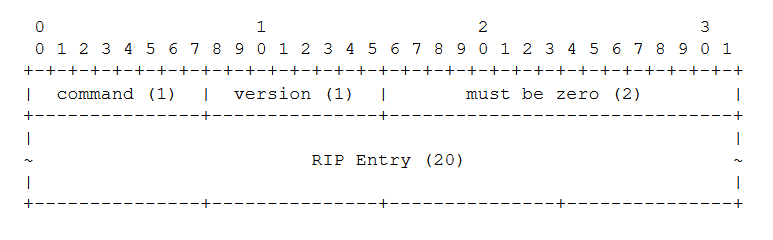
\includegraphics[width=\linewidth]{Graphics/RIPv12_packet.PNG}
  \caption{RIPv1 und RIPv2 Paketformat}
  \label{fig:packet}
\end{figure}

\begin{figure}[ht] 
  \centering
     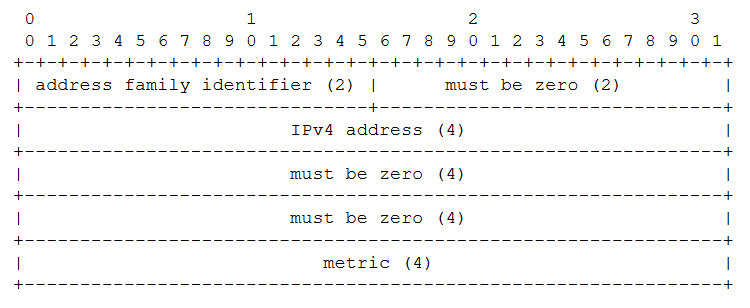
\includegraphics[width=\linewidth]{Graphics/RIPv1_entry.PNG}
  \caption{RIPv1 Eintrag}
  \label{fig:entry1}
\end{figure}

\begin{figure}[ht] 
  \centering
     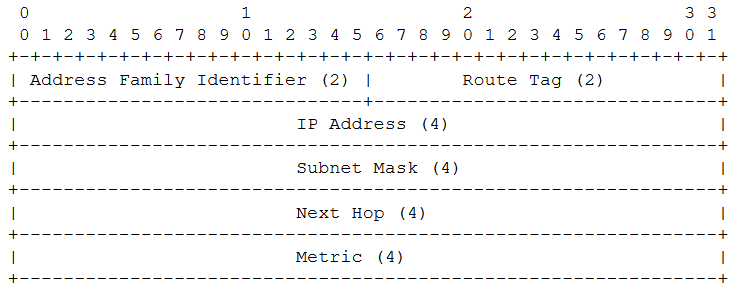
\includegraphics[width=\linewidth]{Graphics/RIPv2_entry.PNG}
  \caption{RIPv2 Eintrag}
  \label{fig:entry2}
\end{figure}
% Um eine Ende-zu-Ende Verbindung zwischen Host 1 und Host 2 zu erm�glichen,
% m�ssen zun�chst die entsprechenden Routen eingerichtet werden. Hierzu wird RIPv2
% genutzt.


%TODO RIP erkl�ren, RFC 1058, RFC 2453
%TODO Verbindungen testen, Routingtabellen, debug RIP, Reflection (Step 12)